% ============================================================================
%  Federated and meta-learned blood-glucose forecasting across sites
%  PLOS Digital Health submission (PLOS template v3.8 Apr 2026)
%
%  STATUS: Full coherent draft. Abstract, Author summary, Introduction,
%  Materials and methods, Results (incl. finetuning), and Discussion (incl.
%  external-comparison subsection) written. Under reviewer-style revision.
%
%  NOTE: this uses the PLOS class options and the `cite` package (numeric
%  Vancouver citations). The bibliography style is `plos2015` (the genuine PLOS
%  Vancouver BibTeX style; the current template ships an identical file renamed
%  plos2025.bst). plos2015.bst is committed alongside this .tex so it compiles
%  as-is on Overleaf. The bib database is references.bib.
% ============================================================================
\documentclass[10pt,letterpaper]{article}
\usepackage[top=0.85in,left=2.75in,footskip=0.75in]{geometry}

\usepackage{amsmath,amssymb}
\usepackage{changepage}
\usepackage{textcomp,marvosym}
\usepackage{cite}
\usepackage{nameref,hyperref}
\usepackage[right]{lineno}
\usepackage[nopatch=eqnum]{microtype}
\DisableLigatures[f]{encoding = *, family = * }
\usepackage[table]{xcolor}
\usepackage{array}

\newcolumntype{+}{!{\vrule width 2pt}}
\newlength\savedwidth
\newcommand\thickcline[1]{%
  \noalign{\global\savedwidth\arrayrulewidth\global\arrayrulewidth 2pt}%
  \cline{#1}%
  \noalign{\vskip\arrayrulewidth}%
  \noalign{\global\arrayrulewidth\savedwidth}%
}
\newcommand\thickhline{\noalign{\global\savedwidth\arrayrulewidth\global\arrayrulewidth 2pt}%
\hline
\noalign{\global\arrayrulewidth\savedwidth}}

% Text layout
\raggedright
\setlength{\parindent}{0.5cm}
\textwidth 5.25in
\textheight 8.75in

\usepackage[aboveskip=1pt,labelfont=bf,labelsep=period,justification=raggedright,singlelinecheck=off]{caption}
\renewcommand{\figurename}{Fig}

\bibliographystyle{plos2015}

\makeatletter
\renewcommand{\@biblabel}[1]{\quad#1.}
\makeatother

% Header and Footer with logo
\usepackage{lastpage,fancyhdr,graphicx}
\usepackage{epstopdf}
\pagestyle{fancy}
\fancyhf{}
\rfoot{\thepage/\pageref{LastPage}}
\renewcommand{\headrulewidth}{0pt}
\renewcommand{\footrule}{\hrule height 2pt \vspace{2mm}}
\fancyheadoffset[L]{2.25in}
\fancyfootoffset[L]{2.25in}
\lfoot{\today}

\begin{document}
\vspace*{0.2in}

% Title must be 250 characters or less. Sentence case.
\begin{flushleft}
{\Large
\textbf{Federated and meta-learned blood-glucose forecasting across sites: a domain-generalisation benchmark and a four-institution deployment}
}
\newline
\\
Luyuan Qi\textsuperscript{1},
Paul Taylor\textsuperscript{1},
Rui Sun\textsuperscript{2},
Taiyu Zhu\textsuperscript{3,4},
Jiahao Sun\textsuperscript{5},
Pantelis Georgiou\textsuperscript{6},
Simon Harper\textsuperscript{7},
Kezhi Li\textsuperscript{1*}
\\
\bigskip
\textbf{1} Institute of Health Informatics, University College London, London, United Kingdom
\\
\textbf{2} School of Computing, Newcastle University, Newcastle upon Tyne, United Kingdom
\\
\textbf{3} Department of Biostatistics \& Health Informatics, Institute of Psychiatry, Psychology \& Neuroscience, King's College London, London, United Kingdom
\\
\textbf{4} Department of Psychiatry, University of Oxford, Oxford, United Kingdom
\\
\textbf{5} [Flock.io Ltd]
\\
\textbf{6} Centre for Bio-Inspired Technology, Imperial College London, United Kingdom
\\
\textbf{7} University of Manchester, Manchester, United Kingdom
\\
\bigskip

* ken.li@ucl.ac.uk
% NOTE (author): (a) Taiyu Zhu's affiliation listing to be confirmed with him
% (per Ken's comment); (b) add department for Manchester if wanted;
% (c) PLOS wants each author's ORCID (corresponding author's is mandatory) and a
% CRediT contribution per author, both entered in the submission system.

\end{flushleft}

% Please keep the abstract below 300 words
\section*{Abstract}
Algorithms that forecast blood glucose 30 minutes ahead are used in type~1
diabetes (T1D) to warn of excursions, but a model trained at one centre can
transfer poorly to new patients and sites, and the varied data that would
fix this cannot lawfully be pooled. Federated learning (FL)
trains a shared model without moving raw records. For glucose forecasting, FL
strategies have rarely been compared head-to-head, evaluations seldom
separate accuracy on training cohorts (held-in) from unseen cohorts
(out-of-distribution, OOD), and almost all such work is simulated.
We ran our federation live across four universities instead, with tooling
light enough for small clinics. Using one encoder--decoder transformer, four
T1D cohorts as federated clients ($\approx 5{,}400$ patient-days of CGM) and
three never-seen cohorts as OOD tests (ReplaceBG, BrisT1D, Flair;
$\approx 63{,}000$ patient-days), we benchmarked local
training against federated
averaging (FedAvg), FedProx, meta-learning for domain generalisation (MLDG),
and two personalised-FL methods under a by-patient split over five seeds, at
30 and 60 minutes.

The meta-learned federated model (MLDG) beat local training held-in,
$20.25$ vs $20.49$ mg/dL RMSE at 30 minutes, lower on
every seed, while plain federated averaging only matched it. The privacy
constraint proved nearly free: MLDG came within $0.09$ mg/dL of a
pooled centralised model, under $1\%$ of CGM sensor error,
and tied it at 60 minutes.
Out of distribution, MLDG was the best federated model on all three unseen
cohorts. On ReplaceBG it reached
$21.30$ mg/dL zero-shot, ahead of FedAvg ($21.48$)
and the mean single-cohort model ($21.73$). Finetuning the federated model
on a new site's
patients beat training there from scratch on all three cohorts; on the two
larger ones, finetuning on just $10\%$ of the training patients ($17$ for
ReplaceBG, $10$ for Flair) still beat it.

% Author Summary: 150-200 words, first person.
\section*{Author summary}
People with type~1 diabetes increasingly rely on algorithms that predict their
glucose half an hour ahead. These work well for the patients they were trained
on but can do worse elsewhere, and the data that would fix that sits in
institutions which cannot legally pool raw records. Federated learning lets
them train a shared model while each keeps its data in-house.

We treated four diabetes studies as collaborating sites, compared the main
federated methods, and tested each on three further studies that gave no
training data. The meta-learned shared model beat each site training alone
on three of the four sites and matched it on the fourth. Federation cost almost nothing: it came within $0.09$ mg/dL
of a model trained on all four datasets pooled, less than the sensors' own
error. On unseen studies it did as well as the best single site. A new site
could beat training alone after finetuning the shared model on about a tenth
of its patients where the cohort is large, and a third where it is small.

We ran this across four universities for real, each holding only its own data.
That gives small clinics a practical route to better predictors.

\clearpage
\newgeometry{top=0.85in,left=1in,right=1in,footskip=0.75in}
\linenumbers

% ===========================================================================
\section*{Introduction}

A reliable forecast of where blood glucose will be in 30--60 minutes is
clinically valuable in type~1 diabetes (T1D): it can trigger preemptive
alerts, inform bolus and snack decisions, and close the loop in automated
insulin-delivery systems~\cite{vettoretti2020advanced,bekiari2018ap}. T1D
affects an estimated 8.4~million people
worldwide~\cite{idf2021,gregory2022t1dindex}, who must continually balance
insulin, food, and activity to keep blood glucose within a narrow target
range. Excursions outside that range drive both the acute dangers of
hypoglycaemia and the long-term complications of hyperglycaemia. Continuous
glucose monitoring (CGM), which reports interstitial glucose roughly every
five minutes, is now central to diabetes care and underpins consensus
glycaemic targets such as time in range~\cite{battelino2019tir}. The same
dense data stream makes short-horizon \emph{forecasting} possible.

Glucose forecasters are now accurate on the cohort they were trained on. How
well they transfer to cohorts they never saw is the open
question~\cite{ghimire2024generalize}. Forecasting has progressed from
autoregressive and classical machine-learning models through recurrent
networks~\cite{martinsson2020}, evaluated on standardised datasets and
challenges~\cite{marling2020ohio}, to the
transformer~\cite{vaswani2017attention} and its time-series
variants~\cite{zhou2021informer,wu2021autoformer}, with transformer
forecasters reporting state-of-the-art accuracy on
glucose~\cite{sergazinov2023gluformer} and curated benchmarks standardising
their evaluation~\cite{sergazinov2024glucobench}. But glucose dynamics,
demographics, and devices differ from site to site, and a model can degrade
on populations it did not see in training~\cite{farahmand2025glumind}.
Robust generalisation therefore requires methods that can exploit diversity
across available cohorts while remaining effective on populations not
observed during training.

Large, diverse training data is exactly what is hardest to assemble. CGM
traces are sensitive personal health records, fragmented across hospitals,
trials, device manufacturers, and registries, and data-protection regimes
such as the GDPR and HIPAA restrict moving them between institutions.
Federated learning (FL) addresses this tension~\cite{mcmahan2017fedavg}:
sites train on their own data and exchange only model updates, so a shared
model is learned without any raw record leaving its institution, a
design widely adopted in medical machine
learning~\cite{rieke2020future,sheller2020federated,kaissis2020secure}. Its
central difficulty is statistical heterogeneity: plain federated averaging
degrades when client distributions diverge, motivating variants such as
FedProx~\cite{li2020fedprox} and SCAFFOLD~\cite{karimireddy2020scaffold}.
Most of this work, however, is evaluated in simulation, with the whole
federation executed on a single machine.

Federation removes the need to pool data, but it does not remove domain
shift: real CGM cohorts differ in device generation, demographics,
treatment protocols, and glycaemic regime. A federated model must therefore
still generalise to patients, and even whole cohorts, it never trained on
(domain generalisation)~\cite{zhou2022dgsurvey}, and/or specialise to each
site (personalisation). Meta-learning for domain generalisation (MLDG)
pursues the former by simulating train/test domain shift within each
update, so the model learns to generalise rather than
memorise~\cite{li2018mldg}.

These ideas have reached glucose forecasting only in the \emph{centralised}
setting: a Transformer trained with MLDG on a single large cohort transfers
zero-shot to external cohorts~\cite{zhu2024gpformer}, and a language-model
backbone improves in-cohort accuracy further~\cite{zhu2026glullm}, but both
are trained on data pooled at a single site, precisely what
data-protection regimes prevent a multi-institution consortium from doing.
Our question is what happens when the same objective must be optimised
\emph{without pooling}, and how the federated alternatives compare under
that constraint.

Bringing domain generalisation into federation is an active
area~\cite{li2025fedDGsurvey}. We benchmark two of its method families.
Meta-learning approaches adapt the model-agnostic meta-learning objective
to federation~\cite{chen2018fedmeta,fallah2020perfedavg}. Personalisation
approaches keep a per-client model: APFL learns an adaptive mixture of the
global and a local model~\cite{deng2020apfl}, while Ditto regularises each
client's personal model toward the global one~\cite{li2021ditto}. We
compare MLDG, APFL, and Ditto alongside standard federated averaging
(FedAvg, FedProx) and single-cohort local training.

\textbf{Yet these methods are rarely compared head-to-head for glucose
forecasting.} Evaluations seldom put them on a common task, and rarely
separate the two regimes that matter clinically, accuracy on patients from
the training cohorts (held-in) versus accuracy on entirely unseen cohorts
(out of distribution, OOD), even though a method can behave quite
differently in the two. Closing this gap under a shared protocol is the
main focus of this paper.

A second, more practical gap is that almost all federated glucose work is
simulated rather than deployed: the usual setup treats individual patients
as clients and runs the whole federation on a single machine
\cite{piao2023graph,piao2026gluadfl,darpit2025fedglu,defalco2023federated}.
The pattern is not specific to glucose. Of 612 federated healthcare
studies only $5.2\%$ report a real-life application \cite{teo2024federated},
and of 107 implementation studies only ten involve real-world distributed
clinical settings \cite{li2025challenges}. The exception is Sun et al.\
\cite{sun2025multicontinental}, who deploy a blockchain-enabled federated
glucose model across five cities on three continents, though on in-silico
subjects rather than real patient records. Production FL frameworks can run
across real sites, but they carry dependencies and assumptions ill-suited
to a small clinical consortium. We therefore also ask a feasibility
question: whether a lightweight cross-site federation for CGM forecasting
can be built and run across real machines with minimal tooling.

This paper makes three contributions.

\textbf{First, a controlled domain-generalisation benchmark of federated
strategies for transformer-based glucose forecasting.} Using a common
encoder--decoder transformer, four real adult T1D cohorts as federated
clients, and three held-out cohorts as OOD test sites, we compare the six
strategies above over multiple seeds, reporting held-in and OOD accuracy
separately at the 30- and 60-minute horizons. Data are split strictly
\emph{by patient}, so every reported error measures generalisation to
people the model has never seen, and the architecture is fixed across
strategies, so the comparison isolates the training strategy.

\textbf{Second, a recipe for onboarding a new site: federate, then adapt.} The
benchmark also shows the limit of a shared model. Zero-shot, it transfers
well but, on two of three new sites, does not close the gap to a model
trained on that site's own patients. Treating the federated model as a foundation closes it. Finetuning
the global model on a fraction of a new cohort's own patients beats training
there from scratch, which gives a practical strategy for onboarding new
sites.

\textbf{Third, we run this federation for real across four institutions, rather
than simulating it.} We build, from scratch, a lightweight cross-site FL
system for CGM forecasting: a stateless aggregation server that holds the
global model but no data, and clients that each wrap one dataset,
communicating over HTTP using only the Python standard library. The results
we report were produced by running this system live across four UK
universities (University College London, the University of Manchester,
Newcastle University, and the University of Oxford), exchanging nothing
but model weights over the public internet. This exercises the conditions a
federation faces across separate administrative domains, with separate
hardware, network round-trips between rounds, and no shared filesystem,
rather than the single-host shortcut that almost all federated glucose work
takes.

Taken together, the benchmark shows how to evaluate federated glucose
forecasting, the finetuning results show what a new site should do with the
resulting model, and the deployment shows that a federation of this kind
runs across real institutions, not only in simulation.

% ===========================================================================
\section*{Materials and methods}

\subsection*{Datasets and federation setup}

We use seven type-1 diabetes (T1D) continuous glucose
monitoring (CGM) datasets (see Data and code availability for access routes).
Four serve as the federated clients, HUPA-UCM \cite{hidalgo2024hupaucm},
ABC4D \cite{abc4d_nct}, ARISES \cite{zhu2022arises}, and T1D-UOM
\cite{alsuhaymi2025t1duom}, with \emph{one dataset per client}. Each dataset
originates from a distinct study, population, and device, so a per-dataset
partition makes every client a genuinely different domain rather than an
arbitrary shard of a pooled corpus. This is what lets the federation function as
a test of cross-domain generalisation. The remaining three datasets,
ReplaceBG \cite{aleppo2017replacebg}, BrisT1D \cite{james2025brist1d}, and Flair
\cite{jaeb_flair}, take no part in federated training and are used in two
roles: as held-out, out-of-distribution (OOD) cohorts on which the trained
models are tested zero-shot, and afterwards as new-site targets in the
finetuning experiments, where a trained model is adapted on a cohort's
training patients and evaluated on its held-out test patients. Within
each client, we partition patients
into disjoint train, validation, and test groups, splitting strictly by
patient ID so that no patient contributes data to more than one group. Reported performance therefore measures generalisation to
unseen patients rather than to unseen windows of patients already observed.

Five of the seven cohorts are obtained through MetaboNet
\cite{wolff2026metabonet}, a recently released resource that consolidates
public T1D datasets into a single harmonised schema on a common 5-minute grid.
These are the clients HUPA-UCM and T1D-UOM, and all three held-out cohorts
(ReplaceBG, BrisT1D, and Flair). The remaining two client cohorts, ABC4D and
ARISES, are converted into the same schema from their original releases.
MetaboNet leaves the grid empty between readings, and our pipeline fills short
gaps and flags them. One cohort, HUPA-UCM, arrives already interpolated
upstream. We handle both cases explicitly (see Data quality below). Patient
counts in
Table~\ref{tab:datasets} are therefore those of the data release we use, which
for the MetaboNet-derived cohorts are smaller than the totals in the source
publications (22 of the 25 published for HUPA-UCM and 14 of the 17 for
T1D-UOM). We do not adopt MetaboNet's own train/test split, which allows the
same patient to appear in both partitions. Instead we re-split strictly by
patient as described above.

Table~\ref{tab:datasets} summarises each cohort. Mean and standard deviation of
CGM are reported in mg/dL, and time-in-range (TIR) is the fraction of CGM
readings in the clinical 70--180 mg/dL band. Patient-days count real
(non-interpolated) CGM readings on the 5-minute grid, i.e.\ real samples
$\times$ 5 minutes: the four clients together contribute
$\approx 5{,}400$ patient-days of CGM, and the three held-out cohorts a
further $\approx 63{,}000$. For HUPA-UCM and T1D-UOM the
window counts and statistics are those of the cleaned data described under
Data quality.

\begin{table}[!ht]
\centering
\captionsetup{justification=centering,singlelinecheck=on}
\caption{\bf Client and held-out cohorts.}
\label{tab:datasets}
\resizebox{\linewidth}{!}{%
\begin{tabular}{lrrrllrrr}
\thickhline
dataset & patients & patient- & total & CGM device & age & mean CGM & sd CGM & TIR (\%) \\
        & (train/val/test) & days & windows &  & (years) & (mg/dL)  & (mg/dL) & 70--180  \\
\hline
\multicolumn{9}{l}{\emph{federated clients}} \\
HUPA-UCM & 22 (18/2/2) & 876 & 205,849 & Libre 2 & 42 (27--48) & 139.3 & 55.1 & 74.0 \\
ABC4D    & 25 (19/3/3) & 3,093 & 562,043 & Dexcom G5 & 36 (29--46) & 155.1 & 63.4 & 65.5 \\
ARISES   & 12 (8/2/2) & 533 & 126,248 & Dexcom G6 & 40 (30--50) & 160.5 & 63.7 & 63.7 \\
T1D-UOM  & 14 (10/2/2) & 876 & 290,753 & mixed & 50 (32--59) & 151.2 & 58.7 & 70.7 \\
\hline
\multicolumn{9}{l}{\emph{held-out OOD cohorts}} \\
ReplaceBG & 208 (166/21/21) & 44,891 & 9,924,380 & Dexcom G4 & 43 (31--55) & 160.7 & 64.5 & 63.1 \\
BrisT1D   & 19 (15/2/2) & 2,706 & 792,546 & mixed & 22 (21--24) & 157.5 & 60.0 & 68.6 \\
Flair     & 113 (91/11/11) & 15,289 & 2,799,490 & Guardian 3 & 19 (16--22) & 161.6 & 60.4 & 65.7 \\
\thickhline
\end{tabular}}
\begin{center}
{\small The three held-out cohorts take no part in federated training. They
are used as zero-shot OOD test sets (Table~\ref{tab:ood}) and as finetuning
targets (Table~\ref{tab:finetune}). Patients are split by patient ID into
train/validation/test as shown. Patient-days count real (non-interpolated)
CGM readings, i.e.\ real samples $\times$ 5 minutes (see text). Age is the
median (interquartile range), for ABC4D and ARISES as reported in prior
publications on these cohorts~\cite{zhu2023glugan,zhu2022arises} and
otherwise computed from the data release. Mixed-device cohorts: T1D-UOM
spans Libre, Dexcom, and Medtronic platforms (7 of its 14 patients wore a
15-minute sensor); BrisT1D spans Dexcom G6, Libre 2, Guardian 4, and Dexcom
ONE. ARISES is both the highest-glucose and the
smallest client cohort. Patient counts are those of the data release we use
and can be smaller than the totals in the original study publications (see
text). For HUPA-UCM and T1D-UOM the window counts and statistics are after the
cleaning step described in the text.}
\end{center}
\end{table}

\subsection*{Preprocessing and windowing}

Every cohort is on a uniform 5-minute grid. We form supervised examples with a
sliding window of 72 samples (6\,h) of CGM context to forecast the next 12
samples (60\,min), advancing the window one sample at a time (stride~1).
Windows that would bridge a sensor gap longer than 6 samples (30\,min) are
discarded, so every example is contiguous. Gaps of up to 30 minutes are
filled by linear interpolation and the filled samples are flagged. CGM is
normalised with a single \emph{global} mean and standard deviation
($154.04 \pm 61.00$ mg/dL) computed from the four training cohorts of the
original release and shared across all clients. A common normalisation keeps
the global model's input scale identical at every site, which is what allows
weights aggregated across clients to be applied directly to the OOD cohorts.
All models, including the single-cohort models, are trained and evaluated
with this shared constant.
Alongside CGM, each example carries a time-of-day mark encoded as
$(\sin 2\pi\,\mathrm{frac},\ \cos 2\pi\,\mathrm{frac})$, where $\mathrm{frac}$
is the fraction of the day, to expose circadian structure.

\subsection*{Data quality}

Two of the client cohorts were not sampled every five minutes at source, and
we handle them explicitly. HUPA-UCM was recorded with a 15-minute sensor
(FreeStyle Libre~2). The MetaboNet release resamples it to the 5-minute grid
and bridges sensor dropouts by linear interpolation, with no flag, so a naive
reading of the file finds no missing data at all. Some interpolated runs span
up to nine hours. We therefore rebuild HUPA-UCM, and T1D-UOM below, from the
release with one extra step. Any run of constant slope, or of sensor-clamped
values ($\le 40$ or $\ge 400$ mg/dL), longer than 60 minutes is treated as
missing. The series is cut at those points, and any clean stretch shorter
than 280 samples is dropped. For HUPA-UCM this keeps 88\% of the training
samples and 70\% of the test samples, with the same patient splits. T1D-UOM
loses under 2\% of its samples. In T1D-UOM, 7 of the 14 patients wore a
15-minute sensor. MetaboNet places their readings on the 5-minute grid and
leaves the samples in between empty. Our pipeline fills gaps of up to 30
minutes by linear interpolation and flags every filled sample, and in T1D-UOM
28.5\% of samples carry that flag. We use it as follows. The training loss
and the validation loss used for model selection are computed over real
samples only, so an interpolated target contributes no gradient. Test metrics
are computed over every grid sample, unmasked, for all cohorts. The same
masked loss is used when training on the held-out cohorts, where BrisT1D is
the most affected: about 31\% of its training windows have at least one
interpolated sample in the forecast target. For ABC4D and ARISES the
timestamps were rebuilt from the source files, so the time-of-day marks are
exact. ABC4D, ARISES, and the three held-out cohorts are otherwise unchanged.
Fewer than 2\% of their windows contain a run that the 60-minute rule would
remove. The cleaning scripts and the resulting split manifests are released
with the code.

\subsection*{Forecasting model}

The forecaster is a standard Informer-style sequence-to-sequence
(encoder--decoder) Transformer~\cite{zhou2021informer} that maps
the 72-step CGM context to the 12-step horizon, using \emph{full}
(dense) scaled dot-product attention.
Holding this architecture fixed across every client and every federated
strategy is what lets our comparisons isolate the \emph{training} strategy rather
than the model. It uses
$d_{\text{model}}=128$, 8 attention heads, 6 encoder layers, 2 decoder layers,
feed-forward width $d_{\text{ff}}=2048$, ReLU activations, and dropout~$0.05$
($\approx 4.9$\,M parameters). Decoding is single-shot rather than
autoregressive, following the Informer convention~\cite{zhou2021informer}: the
decoder input is a warm-up of the last $\texttt{label\_len}=6$ CGM samples
(30\,min) of the context concatenated with 12 zero placeholders for the horizon,
and the corresponding time-of-day marks are supplied for all 18 decoder
positions, as in GPFormer~\cite{zhu2024gpformer}, so the decoder sees the
calendar time of the steps it must predict but
none of their glucose values. The decoder predicts a single CGM channel ($c_{\text{out}}=1$) and the
model is trained with mean-squared-error (MSE) loss over real target samples
(see Data quality). The model emits a point
forecast only. It produces no predictive-uncertainty estimate (see Limitations).

\subsection*{Federated learning system}

Training is coordinated by a from-scratch, networked federated learning system
in which one institution runs a server and each cohort runs a client
(Fig~\ref{fig:system}). The server
holds the global model weights but never sees any data: at round one it mints a
single seeded set of initial weights and broadcasts them, so every client begins
from byte-identical parameters regardless of hardware. Each round, clients fetch
the current global weights, train locally on their own cohort, and return updated
weights. The server aggregates them by FedAvg and advances to the next round.
Clients communicate with the server over HTTP through a small task
state-machine (train\,$\rightarrow$\,validate\,$\rightarrow$\,test), so the same
protocol carries FedAvg, FedProx, and MLDG without modification. The choice of
strategy is entirely client-side, and the server always performs the same FedAvg
aggregation.

The federation is geographically distributed: the four clients are run at four
different UK institutions (University College London, the University of
Manchester, Newcastle University, and the University of Oxford), with one client
per institution, and the aggregation server hosted at one of the sites. All
coordination happens
over the public internet, so the system exercises the real conditions a clinical
consortium would face (separate administrative domains, separate hardware,
network round-trips between rounds) rather than the shared-memory shortcut that
most federated glucose studies take.

\begin{figure}[!ht]
\centering
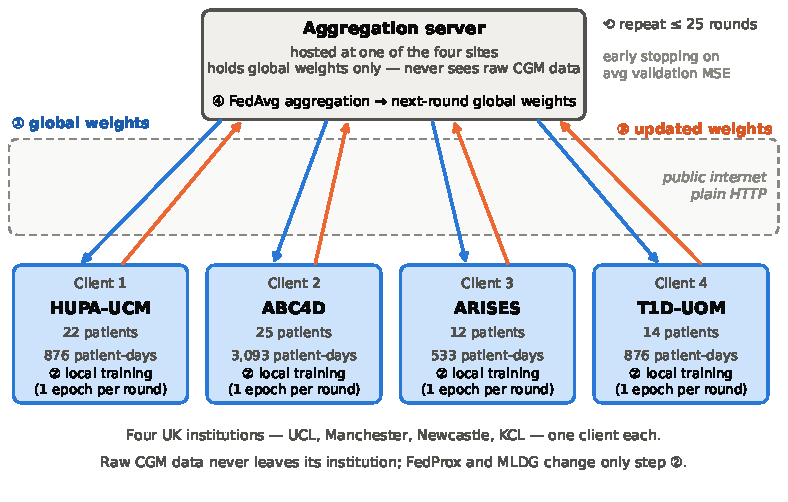
\includegraphics[width=\linewidth]{figures/fl_system.pdf}
\caption{\bf The four-institution federated learning system.
Each communication round, the server broadcasts the current global weights to
the four clients (step 1). Each client trains them on its own cohort for up to
500 gradient steps, at most one epoch (step 2), and returns the updated
weights (step 3). The server
averages the four sets by FedAvg into the next global model (step 4). Rounds
repeat up to a maximum of 25 with early stopping on average validation MSE.
At round one the server broadcasts a single seeded initialisation, so every
client starts from identical parameters. Client boxes give each cohort's size
in patients and in patient-days of real CGM readings (Datasets). All traffic
crosses the public
internet, and raw CGM data never leaves its institution.
FedProx and MLDG change only the clients' local training step, so the same
protocol carries all three strategies.}
\label{fig:system}
\end{figure}

\subsection*{Federated strategies and baselines}

We compare the federated strategies against two baselines: local training and
centralised training.

\textbf{Local baseline.} Our primary comparator is local training: a separate
model trained on a single cohort's data only, with no federation. The central
question of the benchmark is whether federation improves on this baseline,
both when evaluated on the same cohorts that participated (held-in) and on the
unseen OOD cohorts. For OOD we also report the mean over the four single-cohort
models.

\textbf{Centralised baseline.} To measure what the privacy constraint
itself costs, we also train a conventional centralised model on the union of the
four client cohorts, as if their raw data could be pooled at one site. Its
training schedule mirrors the federated one: each of its $50{,}000$ gradient
steps draws one batch from one cohort under a uniformly shuffled schedule
($12{,}500$ steps per cohort, the same per-cohort budget as the federated runs),
with the same architecture, optimiser, batch size, validation-best model
selection, and seeds. This baseline is not available in the setting the paper
addresses, so we
report it not as a competing strategy but as the accuracy federation would have
to match for the privacy constraint to come free.

We implement three federated strategies that train a single global model:
FedAvg, FedProx, and MLDG.

\textbf{FedAvg.} Standard federated averaging~\cite{mcmahan2017fedavg}: the
round protocol of the previous subsection, with plain local training on each
client.

\textbf{FedProx.} FedProx~\cite{li2020fedprox} adds
a proximal term $(\mu/2)\lVert w - w_{\text{global}}\rVert^2$ to each client's
objective to limit client drift. We use $\mu=0.05$.

\textbf{MLDG.} Meta-learning for domain generalisation~\cite{li2018mldg},
adapted to the federated setting~\cite{liu2021feddg}. At each client step, the batch is split by
patient into a meta-train half $S$ and a meta-test half $Q$: whole patients go
to one side or the other, so no patient appears on both, and each side holds
roughly half of the batch's windows (a batch with fewer than two eligible
patients would fall back to a plain gradient step). This never happened in
any MLDG training step in any of the five seeds. Writing
$\mathcal{L}_S$ and $\mathcal{L}_Q$ for the loss on each half and $w$ for the
client's weights, the client first takes a virtual adaptation step on the
meta-train half,
\begin{equation}\label{eq:mldginner}
\tilde{w} \;=\; \mathrm{Adam}\big(w,\ \nabla_w \mathcal{L}_S(w)\big),
\end{equation}
and then updates its actual weights with the gradient of the combined
objective,
\begin{equation}\label{eq:mldgouter}
w \;\leftarrow\; \mathrm{Adam}\big(w,\ \nabla_w\big[\mathcal{L}_S(w) +
\mathcal{L}_Q(\tilde{w})\big]\big),
\end{equation}
where $\mathrm{Adam}(w, g)$ denotes one Adam update of $w$ with gradient $g$.
The model is thereby rewarded for weights that still fit held-out patients
\emph{after} adapting to other patients. The virtual step in
Eq~\eqref{eq:mldginner} is taken by a differentiable copy of the client's Adam
optimiser (via the \texttt{higher} library): it uses the optimiser's current
moment estimates, learning rate, and weight decay, but, being a copy,
writes nothing back. The gradient in Eq~\eqref{eq:mldgouter} keeps the
dependence of $\tilde{w}$ on $w$ (second order, with no first-order approximation)
and is applied by the client's real Adam optimiser. Because the split is over
patients \emph{within} a client, MLDG here simulates cross-\emph{patient}
shift inside a cohort, not the cross-\emph{cohort} shift measured by the OOD
test.

The remaining two strategies are personalised FL methods that create only
local models: APFL and Ditto. Each produces one personalised model per client
and \emph{no} single global model to deploy, so, like the local baseline's
per-cohort models, they are evaluated held-in only and cannot be applied to
the OOD cohorts.

\textbf{APFL.} APFL~\cite{deng2020apfl} learns a per-client
mixture $\alpha v_i + (1-\alpha)w$ of a personal model $v_i$ and the global
model $w$ with an adaptively updated $\alpha$ (initial $0.25$). We also include
a decoupled APFL variant.

\textbf{Ditto.} Ditto~\cite{li2021ditto} trains a personal model
pulled toward the global one by a proximal term ($\mu\in\{0.01,0.1,1.0\}$).

\subsection*{Evaluation protocol and metrics}

We evaluate every strategy in two regimes. \emph{Held-in} performance is measured
on each participating cohort's own held-out patients, isolating predictive
accuracy at the contributing sites. For HUPA-UCM and T1D-UOM these are the
test patients of the cleaned data (Data quality). For HUPA-UCM this makes the
absolute error higher than on the public grid, where long interpolated
stretches are easy to predict. For T1D-UOM the cleaning changes the test error
by less than $0.05$ mg/dL. \emph{OOD} performance is measured on the
three held-out cohorts (ReplaceBG, BrisT1D, Flair), isolating cross-domain
transfer. Only models that exist as one set of weights receive an OOD score:
FedAvg, FedProx, MLDG, the centralised baseline, and each single-cohort
model. We also report the mean of the four single-cohort models as a
reference row.
We report root-mean-squared error (RMSE) in mg/dL as a \emph{point} error at the
30-minute horizon, and use it as the single primary metric for three reasons.
First, it is the unmasked counterpart of the MSE objective every strategy
optimises, so it measures what the training procedures being compared were
asked to do.
Second, 30 minutes is the clinically actionable warning horizon and the one most
widely reported in this literature. Third, this is a benchmark with many
comparisons (nine strategies across four held-in and three OOD cohorts), and
one scalar per strategy and cohort is what keeps those comparisons readable. Because the model
forecasts 12 steps, we also report the 60-minute horizon in full
(Table~\ref{tab:h60}). Neither figure is a window average
over the forecast horizon. Both are the error at that specific step.

\emph{OOD test sets.} In the zero-shot evaluation, every OOD test patient is
unseen in the strong sense: unseen cohort \emph{and} unseen individual. Each
held-out cohort is split by patient in
the same way as the clients, and we score OOD performance on its held-out
\emph{test} patients only (a 21-patient test split for ReplaceBG). Scoring on the
test split rather than the whole cohort is what lets the zero-shot, from-scratch,
and finetuned arms be compared on an identical set of patients per cohort
(Tables~\ref{tab:ood},~\ref{tab:finetune}). Absolute errors still differ across
cohorts for reasons unrelated to our models (device generation, treatment
regimen, and, for Flair, automated insulin delivery, see Discussion), so OOD
errors should be compared \emph{within} a cohort, across strategies, not across
cohorts. All federated and local runs use early stopping on average
validation MSE over real samples (patience~5 over a maximum of 25
communication rounds). Every configuration is repeated over 5 random seeds. We report the mean and standard
deviation across seeds. To test whether a difference between two strategies is
meaningful, we compare their per-seed RMSE with a two-sided paired $t$-test
across the five seeds. We apply the same test to every comparison we report:
held-in, OOD, finetuning against training from scratch, and the data-efficiency
curves.

\emph{Finetuning on held-out cohorts.} The held-out cohorts also serve an
adaptation experiment: is a federated model a better starting point for a new
site than the site's own data alone? For each target cohort we compare three
arms on the same held-out test patients. \emph{Zero-shot} applies a federated
global model unchanged. \emph{From scratch} trains a fresh model of the same
architecture on the target's training patients only, under the same protocol
as a local baseline, including the masked training loss. \emph{Finetuned}
starts from a trained federated global
model (FedAvg, FedProx, or MLDG) and continues training all parameters for
$10$ epochs at learning rate $10^{-4}$ on the target's training patients,
keeping the weights from the epoch with the lowest loss on the target's
validation patients. For the data-efficiency analysis (Fig~\ref{fig:dataeff}),
the finetuning set is restricted to a random $10$--$70\%$ of the target's
training patients, drawn per seed, with the validation and test splits
unchanged.

\subsection*{Implementation and training details}

All models are trained with the Adam optimiser (learning rate~$10^{-4}$, weight
decay~$10^{-3}$, batch size~256, gradient-norm clipping at $1.0$). Each
communication round, a client makes one pass over its local training set,
capped at $500$ gradient steps. The
federated system is implemented in Python using only the standard library for
networking.

\subsection*{Data and code availability, and ethics}

This study is a secondary analysis of de-identified data. It was reviewed and
approved by the University College London Institute of Health Informatics Local
Research Ethics Committee (Project ID 1665, ``Blood glucose prediction modeling
with federated learning using multicentre datasets''). No participants were
contacted and no new human-subjects data were collected. All seven cohorts were
de-identified before we received them and are used under their respective terms
of access. HUPA-UCM \cite{hidalgo2024hupaucm} and T1D-UOM
\cite{alsuhaymi2025t1duom}, together with all three held-out cohorts
(ReplaceBG \cite{aleppo2017replacebg}, BrisT1D \cite{james2025brist1d}, and Flair
\cite{jaeb_flair}), are publicly available through the MetaboNet consolidation
\cite{wolff2026metabonet}. The cleaned HUPA-UCM and T1D-UOM sets used here are
derived from that release by scripts in our repository, which also carries the
split manifests. ABC4D \cite{abc4d_nct} and ARISES
\cite{zhu2022arises} are proprietary clinical-study datasets that the authors
cannot redistribute. They are available upon request and approval by contacting
Dr Kezhi Li (\href{mailto:ken.li@ucl.ac.uk}{ken.li@ucl.ac.uk}). The code for the
federated system and the analysis, together with the exact configuration and
seeds behind each table, is available under the MIT licence at
\url{https://github.com/Luyuannn-unity/fldg-glucose}.
% NOTE (author): optionally mint a Zenodo DOI for the repo at submission and add
% accession numbers/URLs for the public datasets. Confirm the consent phrasing
% ("no participants were contacted") matches what was stated in the LREC
% application; PLOS asks explicitly about consent status. See
% reviews/REQUIRED_FROM_YOU.md items 6-7.

\section*{Results}

Table~\ref{tab:main} reports held-in RMSE on each client's unseen test patients at
the 30-minute horizon. Out-of-distribution performance on
the three held-out cohorts is reported separately in Table~\ref{tab:ood}.

\begin{table}[!ht]
\centering
\captionsetup{justification=centering,singlelinecheck=on}
\caption{\bf Held-in RMSE (mg/dL) at the 30-minute horizon.}
\label{tab:main}
\begin{tabular}{lccccc}
\thickhline
strategy & HUPA-UCM & ABC4D & ARISES & T1D-UOM & avg \\
\hline
Local (per cohort) & $20.44 \pm 0.18$ & $19.75 \pm 0.11$ & $\mathbf{21.87 \pm 0.27}$ & $19.90 \pm 0.19$ & $20.49 \pm 0.09$ \\
\hline
FedAvg  & $20.12 \pm 0.14$ & $19.74 \pm 0.04$ & $22.22 \pm 0.17$ & $19.66 \pm 0.09$ & $20.43 \pm 0.10$ \\
FedProx & $20.36 \pm 0.29$ & $19.87 \pm 0.18$ & $22.35 \pm 0.28$ & $19.76 \pm 0.21$ & $20.58 \pm 0.23$ \\
MLDG    & $\mathbf{19.84 \pm 0.13}$ & $\mathbf{19.53 \pm 0.08}$ & $22.06 \pm 0.11$ & $\mathbf{19.58 \pm 0.08}$ & $\mathbf{20.25 \pm 0.08}$ \\
\hline
APFL           & $20.57 \pm 0.13$ & $19.91 \pm 0.15$ & $22.41 \pm 0.06$ & $19.77 \pm 0.05$ & $20.67 \pm 0.08$ \\
APFL-decoupled & $20.28 \pm 0.15$ & $19.82 \pm 0.12$ & $22.24 \pm 0.18$ & $19.68 \pm 0.12$ & $20.51 \pm 0.12$ \\
Ditto ($\mu{=}0.01$) & $20.15 \pm 0.25$ & $19.69 \pm 0.08$ & $22.15 \pm 0.27$ & $19.61 \pm 0.17$ & $20.40 \pm 0.19$ \\
Ditto ($\mu{=}0.1$)  & $20.19 \pm 0.23$ & $19.68 \pm 0.08$ & $22.14 \pm 0.23$ & $19.60 \pm 0.14$ & $20.40 \pm 0.16$ \\
Ditto ($\mu{=}1.0$)  & $20.24 \pm 0.08$ & $19.72 \pm 0.08$ & $22.23 \pm 0.12$ & $19.66 \pm 0.09$ & $20.46 \pm 0.08$ \\
\hline
\multicolumn{6}{l}{\emph{centralised baseline (pools all four cohorts' raw data)}} \\
Centralised & $19.92 \pm 0.31$ & $19.64 \pm 0.12$ & $21.69 \pm 0.21$ & $19.40 \pm 0.17$ & $20.16 \pm 0.18$ \\
\thickhline
\end{tabular}
\begin{center}
{\small Mean $\pm$ standard deviation across 5 random seeds.
\emph{avg} is the \emph{unweighted} mean of the four cohort means (cohorts differ
in size, so it is not a window-weighted average), reported with the standard
deviation of the per-seed average. Local held-in is each cohort's own
single-cohort model. HUPA-UCM and T1D-UOM are scored on the cleaned test sets
described in Methods. Bold marks the lowest value per column excluding the
centralised baseline, which pools raw data and is unavailable in our setting
(see text).}
\end{center}
\end{table}

\paragraph{The meta-learned federated model beats local training held-in.
Plain averaging matches it.} On the contributing cohorts, the global MLDG
model is more accurate than cohort-specific local training
(Table~\ref{tab:main}). On the held-in average, MLDG is $0.23$ mg/dL below
local training ($20.25$ vs $20.49$), lower on all five seeds (paired
$t$-test, $p = 0.014$). FedAvg is $0.05$ mg/dL below, which is not
significant ($p = 0.14$), and FedProx is level ($p = 0.30$). The MLDG gain is
not spread evenly. It is largest on HUPA-UCM ($0.60$ mg/dL, $p = 0.005$),
present on ABC4D ($0.21$, $p = 0.006$) and T1D-UOM ($0.32$, $p = 0.011$),
and reversed on ARISES, where local training is ahead by $0.19$ mg/dL,
though not significantly ($p = 0.24$). Without HUPA-UCM the average MLDG gain
is about $0.1$ mg/dL. So federation improves in-domain accuracy by a small
but consistent margin, but only with the meta-learned training rule. Plain
averaging matches local training.

\paragraph{Out of distribution, MLDG is the best federated model and beats
the average single cohort.} We test transfer on three
independent held-out cohorts, ReplaceBG, BrisT1D, and Flair
(Table~\ref{tab:ood}). Among the three federated strategies, MLDG has the
lowest error on all three ($21.30$, $26.25$, and $25.02$ mg/dL), ahead of
FedAvg by $0.15$ to $0.23$ mg/dL ($p = 0.014$ on ReplaceBG, $0.027$ on
BrisT1D, $0.09$ on Flair) and level with the centralised baseline. The four
single-cohort models are all stable across seeds (sd $0.09$ to $0.21$). MLDG
beats their mean on every target, by $0.2$ to $0.4$ mg/dL, on all five seeds
($p \le 0.004$). FedAvg beats it on ReplaceBG and matches it on BrisT1D and
Flair, and FedProx matches it on all three. These gains are small next to the measurement error of current CGM
sensors, whose mean absolute relative difference from reference glucose is
$\approx 8$--$9\%$, or roughly $12$--$14$ mg/dL at this population's mean
glucose \cite{garg2022dexcomg7,alva2023libre3}. What the single-cohort rows
add is that held-in accuracy does not predict transfer. The ARISES model, the
worst held-in model of the four, transfers best on BrisT1D and Flair, where it
ties MLDG on the first and edges it by $0.17$ mg/dL on the second. The
HUPA-UCM model transfers worst, $0.7$ to $0.9$ mg/dL behind MLDG on every
target. A
site that ships in one other site's model cannot know in advance which case
it is in. The federated model removes that guess.

\begin{table}[!ht]
\centering
\captionsetup{justification=centering,singlelinecheck=on}
\caption{\bf OOD RMSE (mg/dL) at 30 min on three held-out cohorts.}
\label{tab:ood}
\begin{tabular}{lccc}
\thickhline
model & ReplaceBG & BrisT1D & Flair \\
\hline
\multicolumn{4}{l}{\emph{federated (single deployable global model)}} \\
FedAvg  & $21.48 \pm 0.12$ & $26.48 \pm 0.16$ & $25.18 \pm 0.14$ \\
FedProx & $21.65 \pm 0.21$ & $26.64 \pm 0.28$ & $25.32 \pm 0.22$ \\
MLDG    & $\mathbf{21.30 \pm 0.07}$ & $\mathbf{26.25 \pm 0.12}$ & $\mathbf{25.02 \pm 0.09}$ \\
\hline
\multicolumn{4}{l}{\emph{centralised baseline (pools all four cohorts' raw data)}} \\
Centralised & $21.41 \pm 0.23$ & $26.31 \pm 0.25$ & $25.00 \pm 0.23$ \\
\hline
\multicolumn{4}{l}{\emph{single-cohort (one model per training cohort)}} \\
\;trained on HUPA-UCM & $22.03 \pm 0.16$ & $27.13 \pm 0.21$ & $25.82 \pm 0.18$ \\
\;trained on ABC4D    & $21.49 \pm 0.13$ & $26.47 \pm 0.16$ & $25.19 \pm 0.14$ \\
\;trained on ARISES   & $21.61 \pm 0.13$ & $26.20 \pm 0.19$ & $24.86 \pm 0.09$ \\
\;trained on T1D-UOM  & $21.78 \pm 0.15$ & $26.44 \pm 0.16$ & $25.04 \pm 0.14$ \\
Local (mean of the four) & $21.73 \pm 0.05$ & $26.56 \pm 0.07$ & $25.22 \pm 0.04$ \\
\thickhline
\end{tabular}
\begin{center}
{\small Mean $\pm$ standard deviation across 5 seeds. None of these three cohorts
contributed any training data, so every number is zero-shot transfer to an unseen
cohort \emph{and} unseen patients. Bold marks the lowest value among the
federated strategies. The centralised baseline lands within $0.12$ mg/dL of
MLDG on all three cohorts, with no significant difference, and is excluded
from bolding. Among the single-cohort models, the ARISES model is the lowest
row on BrisT1D and Flair and the HUPA-UCM model is the highest on all three.
\emph{Local} is the unweighted mean of the four single-cohort models above it,
computed per seed. It is the expected error of shipping in one training
cohort's model chosen at random, not a deployable model.}
\end{center}
\end{table}

\paragraph{Zero-shot, the federated model lands among models built on the
target cohort.} Those OOD numbers are absolute errors on cohorts nobody in this
study trained on, so the question is how they compare with models developed on
those cohorts directly. ReplaceBG allows that comparison, because published
results exist for it under our protocol. Our MLDG model reaches $21.30$ mg/dL
there having never seen one of its patients, which places it inside the field of
models trained on ReplaceBG itself. It is ahead of an in-distribution Bi-LSTM,
GRU, ARIMA and SVR, level with N-BEATS, TCN and Crossformer, and behind only
GluLLM and GPFormer, both of which trained on the cohort. GluLLM also consumes
insulin and electronic-health-record inputs we do not use. We set out that
comparison, and its caveats, in the Discussion (Table~\ref{tab:oodprior}).

\paragraph{At the 60-minute horizon the same ordering holds and the gaps
widen.} Because the model forecasts 12 steps, we can read off the 60-minute
horizon as well (Table~\ref{tab:h60}). Errors grow to roughly $1.7\times$
their 30-minute values, as expected, and every qualitative conclusion
survives. MLDG still beats local training held-in (by $0.32$ mg/dL,
$p < 0.001$), FedAvg now does so too (by $0.11$, $p = 0.03$), and FedProx
does not ($p = 0.63$). Ditto still sits at FedAvg's
level and APFL slightly above it. MLDG still has the lowest held-in average
of the three global strategies and the lowest error on all three OOD cohorts,
and its edge over FedAvg is now significant on every OOD cohort ($0.3$ to
$0.5$ mg/dL, $p \le 0.024$). The centralised baseline ties MLDG exactly on
the held-in average ($34.19$ mg/dL), and MLDG is ahead of it on ReplaceBG
($36.38$ vs $36.67$, $p = 0.02$). MLDG still beats the mean single-cohort
model on every unseen cohort, on all five seeds, and FedAvg beats it on
ReplaceBG only.

\begin{table}[!ht]
\centering
\captionsetup{justification=centering,singlelinecheck=on}
\caption{\bf RMSE (mg/dL) at the 60-minute horizon.}
\label{tab:h60}
\resizebox{\linewidth}{!}{%
\begin{tabular}{lcccccccc}
\thickhline
 & \multicolumn{5}{c}{held-in} & \multicolumn{3}{c}{out-of-distribution} \\
strategy & HUPA-UCM & ABC4D & ARISES & T1D-UOM & avg & ReplaceBG & BrisT1D & Flair \\
\hline
Local (per cohort) & $35.94 \pm 0.26$ & $33.82 \pm 0.19$ & $\mathbf{35.84 \pm 0.36}$ & $32.45 \pm 0.15$ & $34.51 \pm 0.03$ & $36.91 \pm 0.04$ & $44.46 \pm 0.10$ & $40.90 \pm 0.06$ \\
\hline
FedAvg  & $35.48 \pm 0.17$ & $33.69 \pm 0.10$ & $36.19 \pm 0.15$ & $32.25 \pm 0.08$ & $34.40 \pm 0.09$ & $36.72 \pm 0.14$ & $44.63 \pm 0.18$ & $41.01 \pm 0.16$ \\
FedProx & $35.62 \pm 0.25$ & $33.70 \pm 0.15$ & $36.32 \pm 0.18$ & $32.27 \pm 0.12$ & $34.48 \pm 0.15$ & $36.83 \pm 0.21$ & $44.70 \pm 0.28$ & $41.12 \pm 0.24$ \\
MLDG    & $\mathbf{35.11 \pm 0.11}$ & $\mathbf{33.37 \pm 0.12}$ & $36.11 \pm 0.10$ & $32.19 \pm 0.08$ & $\mathbf{34.19 \pm 0.07}$ & $\mathbf{36.38 \pm 0.03}$ & $\mathbf{44.17 \pm 0.06}$ & $\mathbf{40.71 \pm 0.06}$ \\
\hline
APFL           & $35.77 \pm 0.17$ & $34.04 \pm 0.31$ & $36.07 \pm 0.10$ & $32.20 \pm 0.08$ & $34.52 \pm 0.11$ & --- & --- & --- \\
APFL-decoupled & $35.59 \pm 0.14$ & $33.89 \pm 0.18$ & $36.12 \pm 0.07$ & $32.25 \pm 0.05$ & $34.46 \pm 0.07$ & --- & --- & --- \\
Ditto ($\mu{=}0.01$) & $35.54 \pm 0.24$ & $33.56 \pm 0.10$ & $36.14 \pm 0.16$ & $\mathbf{32.16 \pm 0.07}$ & $34.35 \pm 0.13$ & --- & --- & --- \\
Ditto ($\mu{=}0.1$)  & $35.56 \pm 0.22$ & $33.54 \pm 0.07$ & $36.14 \pm 0.15$ & $32.17 \pm 0.08$ & $34.35 \pm 0.12$ & --- & --- & --- \\
Ditto ($\mu{=}1.0$)  & $35.58 \pm 0.10$ & $33.62 \pm 0.07$ & $36.21 \pm 0.12$ & $32.22 \pm 0.04$ & $34.41 \pm 0.04$ & --- & --- & --- \\
\hline
\multicolumn{9}{l}{\emph{centralised baseline (pools all four cohorts' raw data)}} \\
Centralised & $35.58 \pm 0.26$ & $33.36 \pm 0.15$ & $35.85 \pm 0.15$ & $31.98 \pm 0.10$ & $34.19 \pm 0.11$ & $36.67 \pm 0.20$ & $44.32 \pm 0.24$ & $40.78 \pm 0.19$ \\
\thickhline
\end{tabular}}
\begin{center}
{\small Mean $\pm$ standard deviation across 5 random seeds. \emph{avg} is the
unweighted mean of the four cohort means, reported with the standard deviation
of the per-seed average. \emph{Local} OOD is the unweighted mean of the four
single-cohort models, computed per seed. The personalised strategies (APFL,
Ditto) deploy per-client models and so have no OOD entries. The centralised
baseline pools raw data and is unavailable in our setting. Bold marks the
lowest value per column excluding the centralised baseline. The 60-minute
values come from the same runs as Table~\ref{tab:main}.}
\end{center}
\end{table}

\paragraph{MLDG has the lowest error in every comparison, and its edge is
significant.} Among the federated strategies that produce a deployable global
model (FedAvg, FedProx, MLDG), MLDG has the lowest error in \emph{every}
held-in and OOD cell at both horizons (16 cells, counting the held-in
average). On the held-in average it
beats FedAvg on all five seeds, by $0.18$ mg/dL at 30 minutes ($t = -4.6$,
$p = 0.010$) and $0.21$ mg/dL at 60 minutes ($t = -7.1$, $p = 0.002$). It
beats FedProx by $0.33$ and $0.29$ mg/dL ($p = 0.017$ and $0.006$). Out of
distribution its gap to FedAvg is $0.15$ to $0.23$ mg/dL at 30 minutes and
$0.3$ to $0.5$ mg/dL at 60 minutes, significant in five of the six cells
(Flair at 30 minutes is the exception, $p = 0.09$). The effect is small in
absolute terms but consistent, and at 30 minutes it is larger than the gain
of FedAvg over local training ($0.18$ vs $0.05$ mg/dL). FedAvg and FedProx
do not differ reliably ($p = 0.06$ at 30 minutes), so we do not rank those
two. The personalised methods do not change the held-in picture. Ditto's
averages sit at FedAvg's level, APFL's are above local training's, and
none of them beats MLDG on any cohort at 30 minutes (Table~\ref{tab:main}).
By construction they cannot be deployed on the OOD cohorts.

\paragraph{The personalised methods converge back toward the global model.} The
personalised strategies do more than fail to beat federation. Given the freedom
to choose how much to personalise, they largely choose not to. APFL deploys a
mixture $\alpha v_i + (1-\alpha) w$ of a personal model $v_i$ and the global model
$w$ with $\alpha$ learned during training. Starting from $\alpha = 0.25$, the
learned $\alpha$ falls to $0.02$--$0.08$ by the final round in every seed
(mean over clients), so the deployed model ends up roughly $95\%$ global: APFL's
own adaptive weighting concludes that the personal model is not worth much on this
task. Ditto tells the same story. Its proximal strength $\mu$ controls how
hard the personal model is pulled toward the global one, and the three
settings we ran ($\mu = 0.01$, $0.1$, $1.0$) give the same held-in average
within $0.06$ mg/dL ($20.40$, $20.40$, $20.46$), at FedAvg's level. How much
personalisation is allowed makes no measurable difference, and no Ditto or
APFL setting beats MLDG on any cohort at 30 minutes. Personalisation buys
nothing here. These methods migrate back to the global solution, and they
forfeit the out-of-distribution transfer that only a shared model provides.

\paragraph{Federation costs almost nothing relative to centralised pooling.}
The comparison that motivates federated learning is not only against local
training but against the centralised model one would train if pooling raw data
were allowed. Held-in, the centralised baseline is ahead of the best federated
strategy by $0.09$ mg/dL on average ($20.16$ vs $20.25$,
Table~\ref{tab:main}), a difference that does not reach significance
($p = 0.32$) and that is concentrated on ARISES, the smallest cohort, where
pooling plausibly helps most. At 60 minutes the two tie exactly on the
held-in average ($34.19$ mg/dL, Table~\ref{tab:h60}). Out-of-distribution
the two are level. MLDG is within $0.12$ mg/dL of the centralised baseline on all
three cohorts at 30 minutes, with no significant difference
(Table~\ref{tab:ood}), and is ahead of it on ReplaceBG at 60 minutes
($p = 0.02$). The privacy constraint is therefore nearly free, and the sensor
yardstick above puts a size on ``nearly'': $0.09$ mg/dL is under $1\%$ of the
$12$--$14$ mg/dL error of the CGM sensors these models read from. Relative to
pooling raw data it could not lawfully pool, a federation gives up less
accuracy than the noise floor of its own input, and nothing measurable
out-of-distribution.

\paragraph{A federated model is a better starting point than local training, on
every target.} Zero-shot transfer mostly has a ceiling. Comparing
Table~\ref{tab:ood} against the from-scratch row of Table~\ref{tab:finetune},
both zero-shot MLDG and the centralised baseline are behind a model
trained from scratch on the target's own data on BrisT1D and Flair. On
ReplaceBG the picture reverses. Zero-shot MLDG beats from-scratch training
there ($21.30$ vs $21.45$ mg/dL, $p = 0.018$) and the centralised baseline is level
with it, so the target's own data is not always decisive. A transferred model
can also serve as a starting point. We therefore asked whether the federated
model helps a \emph{new} site that has local data of its own, by finetuning
the global model on the target cohort's training patients and comparing
against a model trained on that cohort from scratch, on all three held-out
cohorts (Table~\ref{tab:finetune}). The result is consistent. On every
target, finetuning a federated model beats training from scratch on the same
data, by $0.3$--$0.5$ mg/dL for the best strategy, on all five seeds
($p \le 0.007$). Eight of the nine strategy-by-target pairs are significant.
The exception is FedAvg on Flair ($p = 0.12$). Which federated strategy
finetunes best differs by cohort, FedProx on ReplaceBG and MLDG on BrisT1D
and Flair, but the three end within about $0.15$ mg/dL of each other, so the
practical message is robust to that choice: pretraining across cohorts helps,
and the aggregation rule matters less once local data are available. Both
arms see identical target data, so the gain is attributable to the federated
initialisation rather than to extra data.

\begin{table}[!ht]
\centering
\captionsetup{justification=centering,singlelinecheck=on}
\caption{\bf Adapting to a new cohort: from scratch vs federated pre-training then finetuning.}
\label{tab:finetune}
\begin{tabular}{lccc}
\thickhline
adaptation of the new site's model & ReplaceBG & BrisT1D & Flair \\
\hline
train from scratch (100\% local) & $21.45 \pm 0.12$ & $26.03 \pm 0.12$ & $24.52 \pm 0.06$ \\
\hline
FedAvg $\rightarrow$ finetune  & $21.10 \pm 0.18$ & $25.75 \pm 0.05$ & $24.37 \pm 0.14$ \\
FedProx $\rightarrow$ finetune & $\mathbf{20.96 \pm 0.10}$ & $25.80 \pm 0.05$ & $24.32 \pm 0.11$ \\
MLDG $\rightarrow$ finetune    & $21.02 \pm 0.08$ & $\mathbf{25.74 \pm 0.06}$ & $\mathbf{24.23 \pm 0.06}$ \\
\thickhline
\end{tabular}
\begin{center}
{\small RMSE (mg/dL) at 30 min on each target cohort's held-out test patients,
mean $\pm$ sd over 5 seeds. Every arm is trained and evaluated on the same
by-patient splits of the target, so the finetuned rows differ from ``from
scratch'' in their starting weights, not in the data seen. Bold marks the lowest value per
column. Finetuning improves over zero-shot transfer too, most on the cohorts where
zero-shot was weakest (BrisT1D $26.25\rightarrow25.74$, Flair
$25.02\rightarrow24.23$, see Table~\ref{tab:ood}).}
\end{center}
\end{table}

\paragraph{A new site needs little of its own data.} How much target data
does that finetuning actually require? We finetuned the MLDG-pretrained model
on random subsets of each target's training patients ($10$, $20$, $30$, $50$,
and $70\%$) and compared against training from scratch on \emph{all} of the
target's patients (Fig~\ref{fig:dataeff}). On ReplaceBG and Flair, finetuning
on $10\%$ of the target patients already beats from-scratch training on
$100\%$, on all five seeds. That $10\%$ is $17$ patients for ReplaceBG and
$10$ for Flair. Beyond $10\%$ the two curves are close to flat, so more target
data buys almost nothing once the federated initialisation is in place. On
BrisT1D, whose training pool is only $15$ patients, $10\%$ is two patients and
matches from-scratch training. The finetuned model pulls ahead from about
$30\%$ of the patients and keeps improving as the fraction rises, because
each added patient is a large share of its data. The practical implication is
direct. A centre joining after training can reach, and exceed, local-only
performance with ten to twenty patients where the cohort is large, and with
about a third of its patients where it is small, so onboarding a new site
does not require a large local data-collection effort.

\begin{figure}[!ht]
\centering
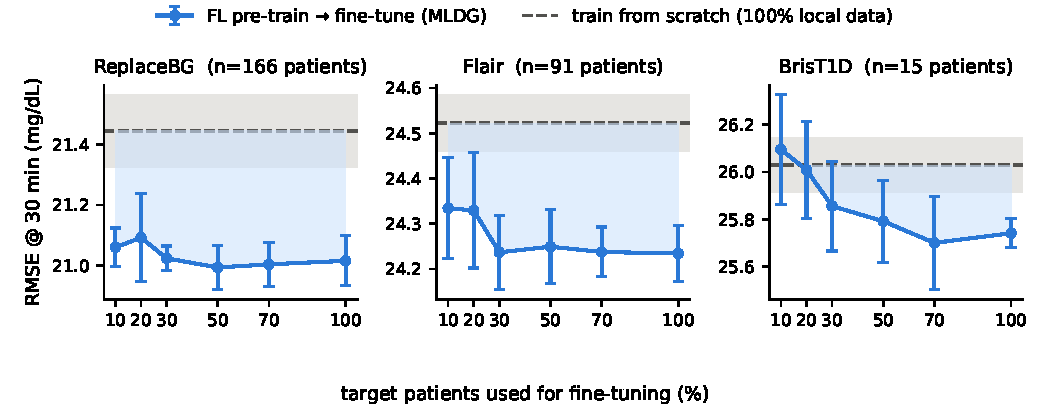
\includegraphics[width=\linewidth]{figures/data_efficiency.pdf}
\caption{\bf Data efficiency of federated pre-training.
Finetuning the MLDG-pretrained model on a fraction of each target cohort's
training patients (blue, mean $\pm$ sd over 5 seeds) against training from scratch
on $100\%$ of that cohort's patients (grey dashed, with its seed-sd band). On
ReplaceBG and Flair, finetuning on $10\%$ of target patients already beats
from-scratch training on the full cohort. On BrisT1D the finetuned model pulls
ahead from about $30\%$. The shaded region marks where finetuning wins.
Training-patient counts: ReplaceBG $166$, Flair $91$, BrisT1D $15$ (so $10\%$
is $17$, $10$, and $2$ patients respectively).}
\label{fig:dataeff}
\end{figure}

\section*{Discussion}

\paragraph{Principal findings.} We federated four real adult T1D cohorts as
distinct domains and tested on three never-seen cohorts (out-of-distribution,
OOD). The meta-learned federated model beat single-cohort local training
in-domain and transferred about as well as the best single cohort out of it,
and better than the average one. Held-in, MLDG was more accurate than local
training (average RMSE $20.25$ vs.\ $20.49$ mg/dL at 30 minutes, on five of
five seeds), plain FedAvg matched it ($20.43$), and MLDG came within $0.09$
mg/dL of
a convergence-matched centralised model trained on the four cohorts pooled
($20.16$), a gap that is not significant and closes to zero at 60 minutes.
So the accuracy cost of never pooling raw data was smaller than the error of
the sensors the model reads from. Among the three global federated
strategies (FedAvg, FedProx, MLDG), MLDG was the most accurate in every
held-in and OOD comparison, and its edge over FedAvg was larger than FedAvg's
edge over local training. OOD, MLDG beat the average single-cohort model on
every held-out cohort, FedAvg and FedProx matched it, and a cohort's in-domain
accuracy did not predict how well its model transferred. These results were produced by a federation that ran across
four universities, UCL, Manchester, Newcastle, and Oxford, training FedAvg,
FedProx, and MLDG under the same protocol over the public internet, with no
raw data leaving any site. It is a working multi-institution system, not a
simulation.

\paragraph{Meta-learned federation gains in-domain and removes the need to
pick a source cohort.} The first benefit is in-domain accuracy, and it comes
with the training rule. MLDG is $0.23$ mg/dL below local training on the
held-in average, on every seed, while FedAvg is $0.05$ below, which is not
significant, and FedProx is level. The MLDG gain is largest on HUPA-UCM,
present on ABC4D and T1D-UOM, and reversed on ARISES, so it is small in
absolute terms and uneven across sites, but it is consistent. The second
benefit is out of distribution. The four single-cohort models transfer
differently, with a spread of $0.5$ to $1.0$ mg/dL between the best and the
worst on each held-out cohort, and
held-in accuracy does not tell them apart. The ARISES model, the least
accurate at home, transferred best on two of the three cohorts, and the
HUPA-UCM model transferred worst on all three. A site that ships in one other
site's model cannot know in advance which it is getting. MLDG beat the
average single-cohort model on all three independent held-out cohorts, on
every seed, and FedAvg and FedProx matched it, a replicated pattern, not a
one-off. This is not a guarantee (three held-out cohorts do
not cover the space of distribution shift, see Limitations). But in a
clinical setting, where distribution shift is inevitable, a model that
transfers well without a guess about which source cohort to trust is a
practical argument for federation, on top of the in-domain gain.

\paragraph{Personalisation did not help.} The personalised strategies
(Ditto, APFL) were given the freedom to trade the global model for a local
one, and they did not use it. APFL's learned mixing weight fell to a $95\%$
global model, Ditto's three settings were indistinguishable, and none of
them beat MLDG on any cohort at 30 minutes, including ARISES, the smallest
and hardest cohort, where only local training came out ahead of MLDG, and
not significantly. These methods also
produce no single global model, so they cannot serve the OOD cohorts at all.
The remaining gap is elsewhere. Zero-shot, the shared model is behind a
model trained on the target's own patients on two of the three held-out
cohorts. The way to close that gap is to treat the global model as a
foundation and adapt it locally.

\paragraph{Finetuning a federated model for a new site.} The finetuning
experiments make the ``foundation-then-adapt'' recipe concrete, and the
pattern holds on all three held-out cohorts (Table~\ref{tab:finetune}). On
every target, the best finetuned federated model beats training from scratch
by $0.3$--$0.5$ mg/dL, on every seed, and improves on zero-shot transfer, most
where zero-shot was weakest. Two points follow. First, a site's own data
trained in isolation did not beat the best finetuned federated model on any
cohort. Together with the held-in gain, that is the evidence that the shared
model adds something a single site cannot recover from its own data alone.
Second, which federated strategy finetunes best depends on the cohort
(FedProx on ReplaceBG, MLDG on BrisT1D and Flair), but the three end within
about $0.15$ mg/dL of each other. So the aggregation rule matters most for
zero-shot transfer and matters less once local data are available. The
data-efficiency analysis (Fig~\ref{fig:dataeff}) adds the practical point.
On the two larger cohorts a new site reaches, and passes, local-only
performance with about $10\%$ of its patients, ten to twenty people. On the
smallest cohort it does so from about $30\%$. So the recipe does not need a
large local dataset. Beyond that point, more target data helps little where
the pool is already large (ReplaceBG, Flair) and still helps where it is
small (BrisT1D). In short: federate to get a shared model, then adapt it to
a new centre with a modest amount of that centre's own data.

\paragraph{On meta-learning.} MLDG's edge is small in absolute terms but
consistent and, at five seeds, significant held-in and on five of six OOD
cells. Its mechanism is worth a note. Our MLDG splits patients into
meta-train and meta-test \emph{within} each client, so it simulates
cross-\emph{patient} shift inside a cohort, not the cross-\emph{cohort} shift
the OOD test measures. That it still comes out ahead OOD is unexplained. A
federated-DG formulation that meta-splits \emph{across} clients would target
the evaluated shift more directly and is the natural next step. At 30
minutes the choice of strategy mattered more than federating at all. Plain
FedAvg gained $0.05$ mg/dL over local training, which is not significant,
FedProx gained nothing, and MLDG gained a further $0.18$ over FedAvg. The
data still dominate, since the centralised model ties MLDG, but the training
rule is not a detail.

\paragraph{Implications for a small group of clinics.} The case for
federating is this: with the meta-learned training rule a centre gains
accuracy on its own patients, and it gets a model that transfers to new
populations without a guess about which source cohort to trust. And since these results were themselves produced by a
four-university federation, there is evidence that the setup is practical,
not hypothetical. Because no raw record leaves any institution, federation
removes the barrier that data-protection rules such as GDPR and HIPAA place
on pooling raw data. Keeping raw data in-house is \emph{necessary but not
sufficient} for compliance: a clinical deployment would add safeguards such as
secure aggregation, access control, and governance and impact assessment.
These are additions to a working architecture, not obstacles to it. With those in
place, the tooling is light enough to run without dedicated
federated-learning infrastructure. We
would expect the benefit to grow as more cohorts join and the shared model
becomes more representative, though we did not vary the number of clients and
cannot show it. Adding cohorts is also the path to something larger: a
foundation model for CGM. General time-series foundation models are already
benchmarked on glucose forecasting, where they do not yet beat a small
supervised LSTM \cite{lu2026glucofmbench}, an argument for training on
more glucose data, not against it. Much of that data is public. Much is not,
and cannot be released. Federation is one route to the part that cannot, and
it has not been tried at this scale. Our four-cohort adult T1D model is not
such a model. What we report is one ingredient, a shared model a new site
can adapt with a small share of its patients, not evidence that the larger
one would work.

\paragraph{Strengths.} Three features set this study apart from prior
federated glucose work. First, it compares local training, FedAvg, FedProx,
MLDG, and two personalised-FL families on one task under one protocol, rather
than reporting a single method in isolation. Second, it separates held-in
from OOD performance, a distinction prior evaluations rarely make
explicit, and an informative one. In-domain, the meta-learned federated
model beats both local training and plain averaging. OOD, federation transfers
without the guess a single-cohort model requires, and the same strategy stays
ahead. Third, the cohorts are split strictly by patient and normalised
with a single shared statistic, and the federation ran across four real
institutions in separate administrative domains rather than as shards of one
dataset on one host. To our knowledge these are the first federated
glucose-forecasting results from a multi-institution run on real patient data.

\paragraph{Positioning against prior results on these cohorts.} Our
per-cohort accuracy is competitive with published results on the same
datasets, under a harder protocol. The difference is the train/test split.
Almost all prior work splits each patient's series in time, the first
portion for training and the last for testing (a \emph{by-time} split), so
every test window comes from a patient the model has already seen. We split
\emph{by patient}: test patients are disjoint from training patients, so every
reported number measures generalisation to people the model has never seen.
By-patient evaluation is the harder task and the one that matches deployment,
where a predictor meets new patients, but it typically yields higher error
than a by-time split on the same cohort. Table~\ref{tab:prior} collects the
closest external results. On HUPA-UCM and T1D-UOM, the strongest real-data
RMSE@30 baselines are from GlucoFM-Bench \cite{lu2026glucofmbench} (a
benchmark of time-series foundation models, univariate CGM, by-time split):
HUPA-UCM 16.71 and T1D-UOM 20.81 mg/dL. On ARISES and ABC4D they are from the
personalised meta-learning forecaster of Zhu et al.\ \cite{zhu2023fcnn} (CGM
plus carbohydrate and insulin, by-time split): 20.23 and 20.25 mg/dL. Our
by-patient figures for a global model (MLDG, our best federated strategy:
HUPA-UCM 19.84, ABC4D 19.53, ARISES 22.06, T1D-UOM 19.58 mg/dL) sit in the
same 17--22 mg/dL range despite the harder split. On ARISES and ABC4D they do
so using CGM alone, against models that also use insulin and carbohydrate
inputs. On HUPA-UCM our test set is harder still, because we removed the
long interpolated stretches of the public release that are trivially
predictable (Data quality). We do not claim to beat these numbers. A
by-patient result is not expected to. We claim to match them under an
evaluation that better reflects deployment. To our knowledge no prior paper reports all four
of these cohorts, separates held-in from out-of-distribution performance, or
evaluates across-patient generalisation as we do. The one prior work that
also splits by patient (AEGIS \cite{pansheriya2026aegis}, on T1D-UOM via
leave-one-patient-out) forecasts only to 15 minutes, so it is not comparable
at our 30-minute horizon.

\begin{table}[!ht]
\centering
\captionsetup{justification=centering,singlelinecheck=on}
\caption{\bf Published RMSE@30 on our cohorts, with split protocol.}
\label{tab:prior}
\begin{tabular}{lllll}
\thickhline
study (best model) & cohort & RMSE@30 (mg/dL) & split & sd over \\
\hline
GlucoFM-Bench \cite{lu2026glucofmbench} (LSTM) & HUPA-UCM & 16.71 (4.82) & by-time & patients \\
GlucoFM-Bench \cite{lu2026glucofmbench} (LSTM) & T1D-UOM  & 20.81 (4.26) & by-time & patients \\
Zhu et al.\ \cite{zhu2023fcnn} (FCNN)          & ARISES   & 20.23 (3.38) & by-time & patients \\
Zhu et al.\ \cite{zhu2023fcnn} (FCNN)          & ABC4D    & 20.25 (2.60) & by-time & patients \\
\hline
Ours (MLDG, global)            & HUPA-UCM & 19.84 (0.13) & \emph{by-patient} & seeds \\
Ours (MLDG, global)            & ABC4D    & 19.53 (0.08) & \emph{by-patient} & seeds \\
Ours (MLDG, global)            & ARISES   & 22.06 (0.11) & \emph{by-patient} & seeds \\
Ours (MLDG, global)            & T1D-UOM  & 19.58 (0.08) & \emph{by-patient} & seeds \\
\thickhline
\end{tabular}
\begin{center}
{\small A \emph{by-time} split tests on later windows of patients seen during
training. A \emph{by-patient} split tests on entirely unseen patients and is the
harder, deployment-relevant task. External sd is across patients, ours across
5 seeds. Numbers are indicative, not head-to-head, because the split (and, for
Zhu et al., the input features) differ. Our HUPA-UCM test set also excludes
the upstream-interpolated stretches of the public release, so it is harder
than the benchmark's: our models score about 1.4 mg/dL lower on the public
grid, averaged over strategies. Other papers on these cohorts report
non-comparable metrics or horizons: Tan \& McBeth \cite{tan2026uncertainty}
(MARD only), AEGIS \cite{pansheriya2026aegis} (15-min horizon, mmol/L),
Manchanda et al.\ \cite{manchanda2025lstm} (window-averaged RMSE), and Kolev
et al.\ \cite{kolev2026benchmark} (synthetic data only).}
\end{center}
\end{table}

\paragraph{Zero-shot transfer is competitive with models trained on the target
cohort.} The comparison above concerns the cohorts we trained on. The sharper
test is a cohort we have \emph{never seen}, against models developed on it.
ReplaceBG allows this comparison: two studies report 30-minute RMSE on it
under the same protocol we use: a by-patient hold-out, on a 5-minute grid,
as a point error at the 30-minute horizon. The only difference is that they
trained on ReplaceBG and we did not (Table~\ref{tab:oodprior}). Our federated
MLDG model reaches $21.30$ mg/dL on ReplaceBG having never seen any of its
patients. That places it inside the field of models developed on the cohort.
It beats an in-distribution Bi-LSTM ($21.7$), GRU ($22.1$), ARIMA ($28.1$)
and SVR ($37.4$), and is level with N-BEATS ($21.2$), TCN ($21.3$) and
Crossformer ($21.1$). It trails only GluLLM ($20.6$, which also uses insulin
and electronic-health-record features we do not) and GPFormer ($19.2$), which
was trained centrally on ReplaceBG itself. Three caveats apply. First, the
$2.1$ mg/dL gap to GPFormer mixes two differences: GPFormer both trained on
the target cohort \emph{and} uses sparse attention where ours uses full
attention, so the gap is not a clean measure of the cost of federation alone.
Second, the test sets are not identical: the published studies evaluate on a
46-subject hold-out from a model \emph{trained on the rest of ReplaceBG}. We
evaluate on a 21-patient test split from a model that never saw \emph{any}
ReplaceBG patient. Both test on unseen individuals. Only ours also faces an
unseen cohort, a different and arguably harder setting. Third, reported
ReplaceBG results vary widely with protocol: one study reports $9.3$ mg/dL
\cite{jaloli2023cnnlstm}, but on a 15-minute grid and with a rolling split
that re-admits test patients to training. That is not comparable to any of
the numbers here. With those caveats, the point stands: a model that never
saw ReplaceBG, and never pooled raw data from anywhere, lands inside the
field of models developed on it.

This parity is specific to the 30-minute horizon. It does not survive at 60
minutes. There, our zero-shot MLDG reaches $36.38$ mg/dL on ReplaceBG
(Table~\ref{tab:h60}) against $32.3$ for GPFormer, $34.1$ for N-BEATS and
$34.7$ for Bi-LSTM \cite{zhu2024gpformer}, behind \emph{every}
in-distribution baseline rather than among them. The likely reason: at short
horizons a forecaster relies on recent CGM dynamics, which transfer across
cohorts, so a model trained elsewhere loses little. At longer horizons
prediction depends more on cohort-specific behaviour (meal and insulin
routines, treatment regimen, sensor characteristics), which a model that
never saw the cohort does not know. Zero-shot federation buys parity where
shared physiology dominates the task, and pays a growing price where
cohort-specific habit dominates. For the 30-minute alerting use case that
motivates this work, the first regime is the relevant one. For longer-range
planning, local data are worth more.

\begin{table}[!ht]
\centering
\captionsetup{justification=centering,singlelinecheck=on}
\caption{\bf Our zero-shot result on ReplaceBG against models trained on ReplaceBG.}
\label{tab:oodprior}
\begin{tabular}{llcc}
\thickhline
model & inputs & trained on ReplaceBG & RMSE@30 \\
\hline
GPFormer \cite{zhu2024gpformer}    & CGM                & yes & $19.2$ \\
GluLLM \cite{zhu2026glullm}        & CGM + insulin + EHR & yes & $20.6$ \\
Crossformer \cite{zhu2026glullm}   & CGM + insulin + EHR & yes & $21.1$ \\
N-BEATS \cite{zhu2024gpformer}     & CGM                & yes & $21.2$ \\
TCN \cite{zhu2026glullm}           & CGM + insulin + EHR & yes & $21.3$ \\
\textbf{Ours, MLDG (federated)}   & \textbf{CGM}       & \textbf{no} & $\mathbf{21.30}$ \\
\textbf{Ours, FedAvg}             & \textbf{CGM}       & \textbf{no} & $\mathbf{21.48}$ \\
\textbf{Ours, FedProx}            & \textbf{CGM}       & \textbf{no} & $\mathbf{21.65}$ \\
Bi-LSTM \cite{zhu2024gpformer}     & CGM                & yes & $21.7$ \\
GRU \cite{zhu2026glullm}           & CGM + insulin + EHR & yes & $22.1$ \\
ARIMA \cite{zhu2024gpformer}       & CGM                & yes & $28.1$ \\
SVR \cite{zhu2024gpformer}         & CGM                & yes & $37.4$ \\
\thickhline
\end{tabular}
\begin{center}
{\small RMSE (mg/dL) at the 30-minute horizon on ReplaceBG. All rows use a
by-patient hold-out on a 5-minute grid and report a \emph{point} error at 30
minutes (not a window average). Every published row was \emph{trained on
ReplaceBG}. Our three rows were trained on four entirely different cohorts and
never saw ReplaceBG, so they are zero-shot. Published values are read from
\cite{zhu2024gpformer,zhu2026glullm}. Those two sources evaluate on the same
46-subject hold-out of ReplaceBG, whereas our models are evaluated on a 21-patient
test split of ReplaceBG that, like all ReplaceBG patients, was never seen in
training. Note that GPFormer additionally uses sparse attention while our
forecaster uses full attention, so the GPFormer--ours gap reflects architecture as
well as training regime.}
\end{center}
\end{table}

\paragraph{BrisT1D and Flair are, to our knowledge, previously unbenchmarked.}
We report $26.25$ and $25.02$ mg/dL on these two cohorts but make no
comparative claim: we could find no published 30-minute-horizon RMSE in mg/dL
on either. The BrisT1D Kaggle competition \cite{kaggle2024brist1d} targets a
\emph{60-minute} horizon in mmol/L and so is not comparable, the published
models that use BrisT1D report errors on a normalised scale, and for Flair we
found no glucose-forecasting benchmark at all. We therefore offer these two
numbers as zero-shot reference points for future work rather than as wins.
One property of Flair matters here: it is a hybrid closed-loop (automated
insulin delivery) cohort \cite{bergenstal2021flair}, and automated delivery
suppresses glycaemic variability, which tends to make forecasting easier. Its
lower error relative to BrisT1D partly reflects the cohort rather than the
model. The value of
these two cohorts is not that we beat anyone on them. It is that the
federated models behave consistently on three independent unseen populations,
and that the same strategy, MLDG, stays ahead on each.

\paragraph{Limitations and future work.} Several constraints bound these
conclusions, and each points to a next step.
\emph{(i) Clinical relevance.} Our goal was to establish how federated
strategies compare on the forecasting objective they were trained for, so we
report a single aggregate error (RMSE at 30 and 60 min) and a point forecast with no
calibrated uncertainty. Aggregate RMSE is dominated by the euglycaemic range and
can be near-blind to the safety-critical hypoglycaemic tail, and the studies we
compare against also report clinical error grids (Clarke/Parkes), MARD, or
hypo-/hyperglycaemia detection. Whether federation's small advantage survives
on such metrics is untested. The next step is to train and evaluate with clinical
relevance built in, for example a loss that penalises forecasts falling in
the dangerous zones of the error grid, and to report the full error-grid,
MARD, and event-detection profile with predictive uncertainty.
\emph{(ii) OOD breadth and composition.} Our transfer claim rests on three
held-out cohorts (ReplaceBG, BrisT1D, Flair), and the three are not equivalent
tests. Flair is a hybrid closed-loop (automated insulin delivery) cohort of
adolescents and young adults, whose suppressed glycaemic variability makes
forecasting easier. BrisT1D is a small open-loop young-adult cohort (15
training patients in the release we use). Absolute errors are therefore not comparable \emph{across} the three
cohorts. Only the within-cohort ranking of strategies is. A leave-one-cohort-out
design would probe transfer further.
\emph{(iii) Statistical power and tuning.} Our tests use five seeds on one
fixed patient split, so seed sd understates patient-sampling uncertainty,
and we made no correction for the number of comparisons. The margins we call
significant are small in absolute terms ($0.2$ to $0.6$ mg/dL), and the
held-in gain over local training is concentrated on one cohort (HUPA-UCM).
Some comparisons remain unsettled at this sample size: FedAvg against local
training, MLDG against the centralised baseline, MLDG against FedAvg on
Flair at 30 minutes, and FedAvg against FedProx. FedProx used a single untuned $\mu$. (APFL, by
contrast, is not under-tuned: its mixing weight is learned, and we report
where it converges.)
\emph{(iv) Horizon.} We report the 30- and 60-minute horizons. The model does
not forecast beyond 60 minutes, so the 90- and 120-minute horizons some
comparators report are out of scope. Our parity with in-distribution models on
ReplaceBG holds at 30 minutes but not at 60.
\emph{(v) Privacy guarantees and jurisdiction.} Raw data never moves, and the
next step is to back that property with formal protections such as secure
aggregation and differential privacy, which the current system does not yet
add. All four sites are also within one country, so the legal and governance
complexity of a cross-border federation remains untested. We plan to extend the
four-institution federation across national borders, reporting communication,
latency, straggler, and failure behaviour under cross-jurisdiction governance.
\emph{(vi) Population and inputs.} All seven cohorts are T1D, and all but
Flair are adult, leaving paediatric and type-2 transfer largely untested. The model is CGM-only, so event-aware
inputs such as insulin and carbohydrate information are a natural addition. We
also scope the benchmark to meta-learning and personalisation, leaving
representation-alignment methods to future work.
\emph{(vii) Mechanism.} The centralised baseline shows that federation
recovers the accuracy of pooling, held-in and out of distribution. The main
mechanism should therefore be read as ``more diverse training data, obtained
under a privacy constraint''. The training rule adds a smaller, second
effect, since MLDG beats plain averaging at both horizons.
Finally, our finetuning is a two-stage pipeline (federate, then adapt).
Training the global model and its per-site specialisations \emph{jointly}, and
continual federation as populations and devices drift, are natural extensions
this framework is set up to support.


% ===========================================================================
% Compile references.bib with the plos2025.bst style (ships with PLOS template).
\bibliography{references}

\end{document}
